%! suppress = MissingImport
%If you are using Arduino IDE 1.8, see this \href{https://www.arduino.cc/en/Guide/ArduinoNano#select-your-board-type-and-port}{Tutorial} for selecting the \developmentboard\ board, processor, and COM port (or this \href{https://www.arduino.cc/en/Guide/ArduinoUno#select-your-board-type-and-port}{Tutorial for the Arduino Uno}, which has more detail on selecting the COM port).
If you are using Arduino IDE 1.8, see the Quickstart Guide on the \href{https://docs.arduino.cc/hardware/nano}{\developmentboard's documentation page} for selecting the \developmentboard\ board, processor, and COM port.
If you are using Arduino IDE 2.0 or the Arduino Web Editor, COM port should be automatically detected.
You will still need to select the board and processor;
see Figure~\ref{fig:selecting-mcu} and the discussion in Section~\ref{subsubsec:processor-selection}.

\begin{figure}
    \centering
    \subfloat[Selecting the board with Arduino IDE 1.8.] {
        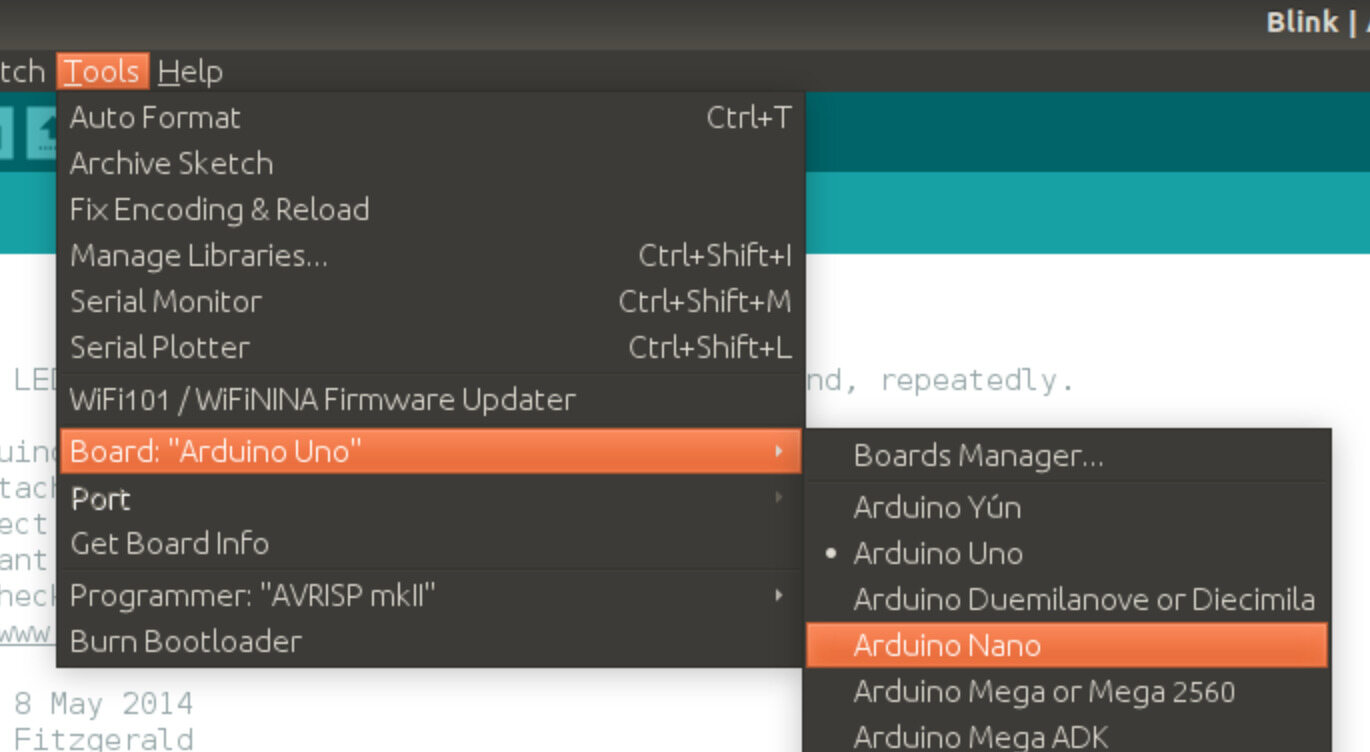
\includegraphics[width=7cm]{microcontroller/ide/selecting-nano-1_8}
%        \label{fig:selecting-board-1}
    }
    \hfil
    \subfloat[Selecting the board with Arduino IDE 2.0.] {
    % 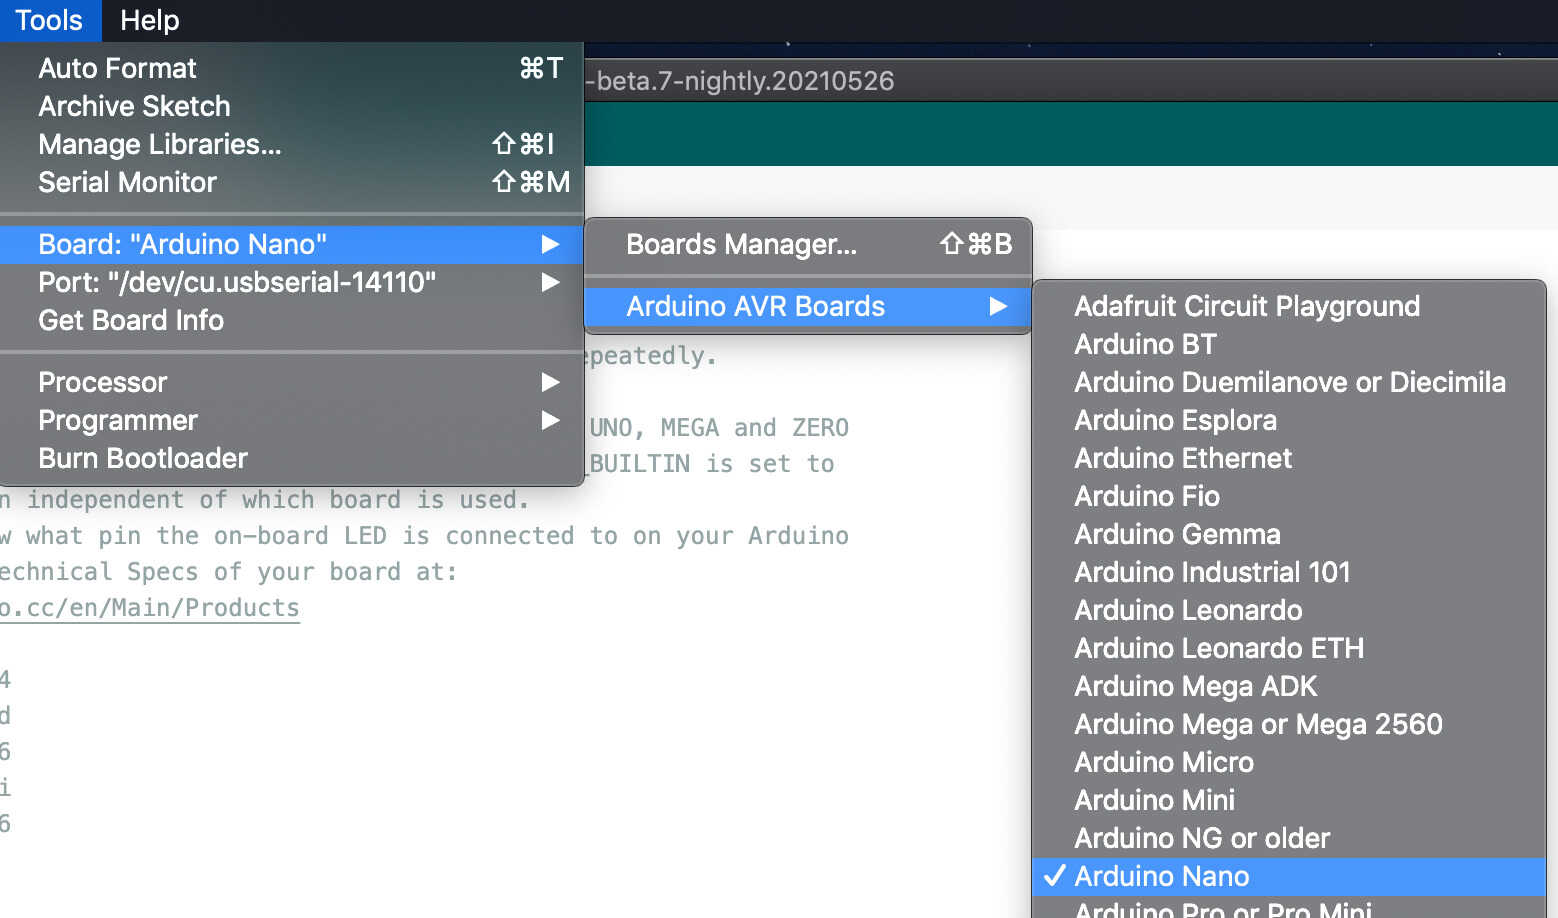
\includegraphics[width=7cm]{selecting-nano-from-menu}
        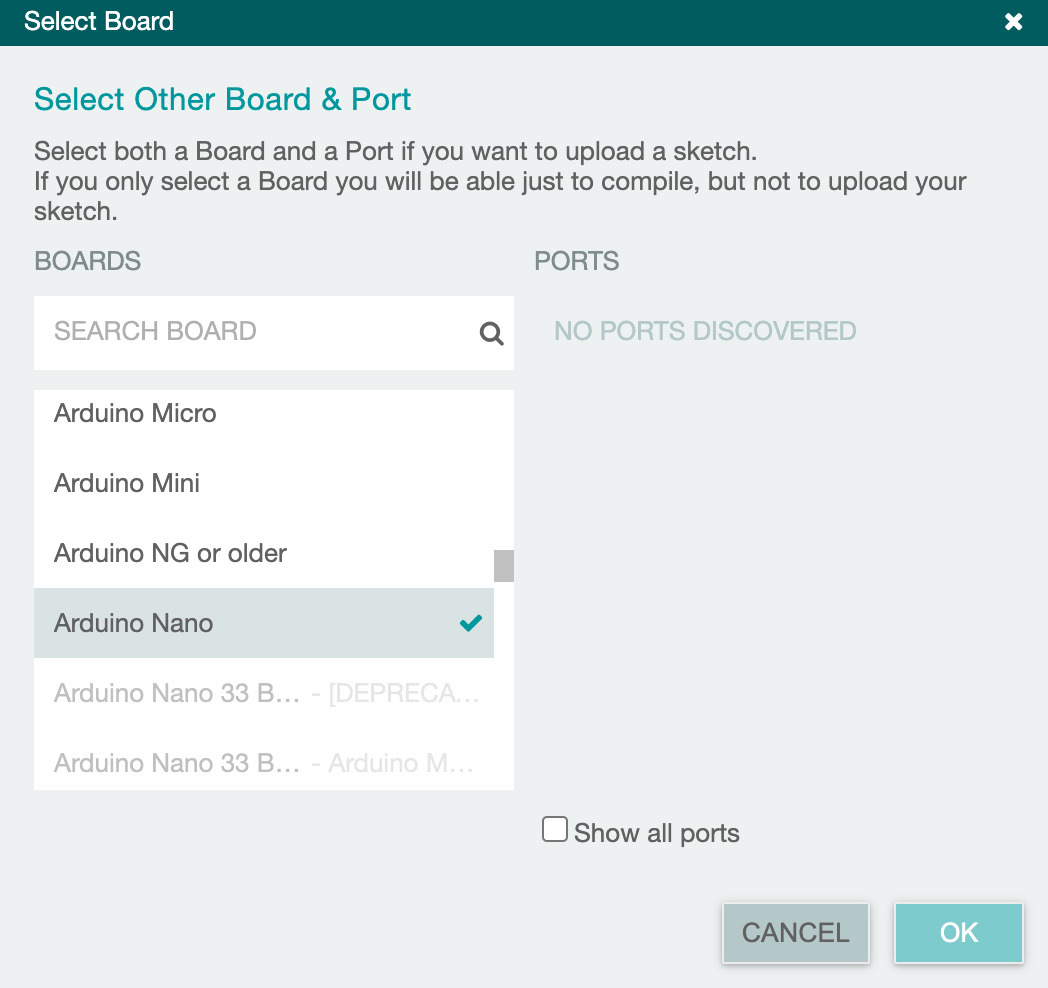
\includegraphics[height=4.1cm]{microcontroller/ide/selecting-nano}
%        \label{fig:selecting-board-2}
    }

    \subfloat[Selecting the processor after selecting the board.] {
    % \vtop{\vskip-4.1cm\hbox{\includegraphics[width=5cm]{selecting-nano-processor}}}
        \includegraphics[width=7cm]{microcontroller/ide/selecting-nano-processor}
        \label{fig:selecting-processor}
    }
    \caption{Selecting board and processor in the Arduino IDE.
    \label{fig:selecting-mcu}}
\end{figure}

\subsubsection{Selecting the Correct ``Processor''}\label{subsubsec:processor-selection}

There are \textit{three} choices for the \developmentboard{}'s processor, two of which specify the ATmega328P processor.
Even though the difference is a USB interface issue, it is resolved through the Arduino IDE's ``Processor'' selection:

\begin{itemize}
    \item Official \developmentboard{}s use the FT232RL USB interface chip.
    Under the ``Tools'' menu, when choosing ``Processor'', select ``ATmega328P''.
    \item \textit{Most} \developmentboard\ clones use the CH340 USB interface chip.
    Under the ``Tools'' menu, when choosing ``Processor'', select ``ATmega328P (Old Bootloader)''.
    (If you are using the Arduino IDE 1.8.4 and earlier, which don't have the ``(Old Bootloader)'' option, simply select ``ATmega328P'').
    \item If you have an older \developmentboard\ that uses the ATmega168 processor, replace it with one that has an ATmega328P processor.
\end{itemize}

\subsubsection{Updating USB Driver if Necessary}

We have seen some Windows computers without the CH340 USB driver.
If you encounter this problem and the Device Manager shows you the warning in Figure~\ref{fig:usb-warning}, then the first thing to try is updating the driver.
Right-click on USB2.0-Ser! (Figure~\ref{fig:update-driver}) and choose ``Update driver''.
Then choose ``Search automatically for updated driver software''.

\begin{figure}
    \centering
    \subfloat[] {
        
\includegraphics[width=.4\textwidth]{microcontroller/usb-drivers/device-manager-warning}
        \label{fig:usb-warning}
    }
    \hfil
    \subfloat[] {
        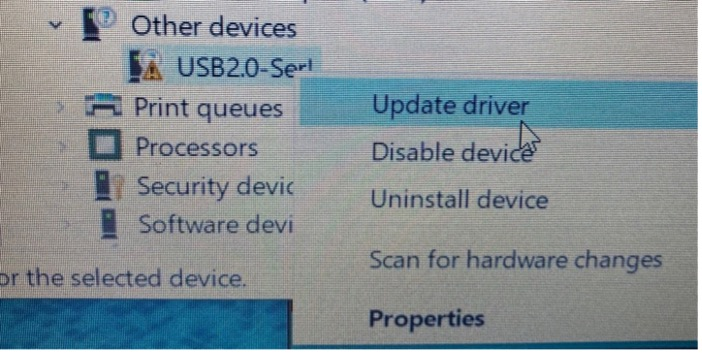
\includegraphics[width=.4\textwidth]{microcontroller/usb-drivers/update-driver}
        \label{fig:update-driver}
    }
    \caption{Some Windows computers lack the CH340 USB driver.}
\end{figure}

If Windows reports that ``Windows has successfully updated your drivers'' then you should now be able to connect to the \developmentboard.
On the other hand, if Windows reports that ``Windows was unable to install your USB2.0-Ser!'', then the \href{https://learn.sparkfun.com/tutorials/how-to-install-ch340-drivers/}{How to Install CH340 Drivers} page at sparkfun.com will guide you through manually downloading the driver and installing it.

Sparkfun's \href{https://learn.sparkfun.com/tutorials/how-to-install-ch340-drivers/}{How to Install CH340 Drivers} page also has instructions for installing the driver on MacOS and on Linux;
however, we are not aware of any students needing to manually install the CH340 driver on MacOS\@.

\subsubsection{No Driver Warning but Cannot Connect}

If you see no warnings but your Windows computer still won't communicate with thhe \developmentboard\, then probably what happened is that your computer has the driver, but you're telling the IDE to connect to the wrong virtual COM port.
The typical way to handle this is to disconnect the \developmentboard\ from your computer, go to the part of the menu where you connect to the COM port, connect the \developmentboard\ to your computer, and select whichever COM port appears after plugging in the \developmentboard.
